\documentclass[../report.tex]{subfiles}
\begin{document}
\graphicspath{{img/}{../img/}}
\label{sec:enums}

When designing the DTOs for the \textit{ShareIt Back End} there was one decision which was particularly impactful.
Since the data model was designed to be as generic as possible a decision needed to be made on how to best reflect this in the DTOs.
The following three approaches were considered.
\begin{itemize}
\item Using inheritance to model the differences between the different entity types.
\item Using strings to represent the different entity types and entity information types.
\item Using enums to represent the different entity types and entity information types.
\end{itemize}

\subsubsection{Inheritance}
Using inheritance to model the differences between different entity types had the advantage of allowing the use of polymorphism to make collections of \textit{Media Item} objects and passing them as result for e.g. the search function. Adding a new type would then simply be a matter of creating a new subtype as depicted on \ref{fig:dto_inheritance}.
 
However, this approach did not take advantage of the flexibility of the data model. The \textit{ShareIt Back End} would have to define which properties each of the different \textit{Media Item}s had, thus forcing the \textit{Client} to use its definition of each type.

\begin{figure}[!h]
\label{fig:dto_inheritance}
\centering
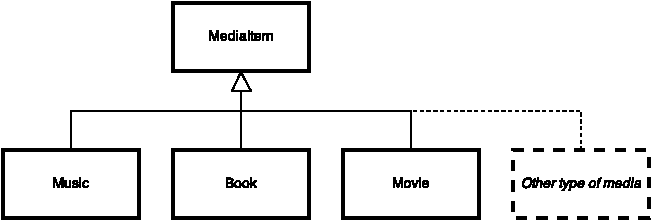
\includegraphics[scale=0.7]{DTOInheritance.pdf}
\caption{DTOs using inheritance}
\end{figure}

\subsubsection{Using strings to represent types}
Using strings to represent the different entity and information types had the advantage of making full use of the flexibility of the data model. The various \textit{Client}s would be able to define their own types simply by deciding on a name for them. 

However, this would potentially be very costly for the services because queries would have to be made for every information to try and match the Type string with an EntityInfoType in the database to retrieve the id which the relation should be made to. If no such id could be found a new EntityInfoType would have to be created and stored. This would be extra cumbersome because spelling wouldn't be ensured across calls and the values \textit{"title"} and \textit{"Title"} would not be the same.
 
\begin{figure}[!h]
\label{fig:dto_types_string}
\centering
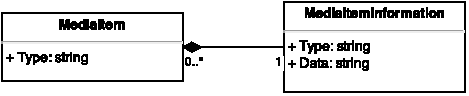
\includegraphics[scale=0.7]{../img/typesAsString.pdf}
\caption{DTOs using strings to represent types}
\end{figure}

\subsubsection{Using enums to represent types}
The middle ground between flexibility and type safety was sought by using enums to represent types instead of strings.
The DTOs were still flexible enough that the \textit{Client}s were able to define which information they wanted each \textit{Media Item} to hold, but it was ensured that the different information could only have a type specified by the \textit{ShareIt Back End}.

In order to support the addition of new types to the database an invariant was enforced making sure that the value of the enums matches the corresponding id in the database. 
This meant that the enums could be cast to integers when saving data in the database and vice versa when retrieving data from the database. 

\begin{figure}[!h]
\label{fig:dto_types_enum}
\centering
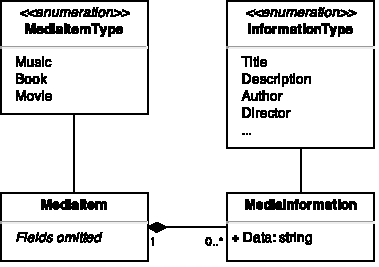
\includegraphics[scale=0.7]{../img/typesAsEnum.pdf}
\caption{DTOs using enums to represent types}
\end{figure}
\end{document}